%\documentclass{acm_proc_article-sp} UNCOMMENT FOR NO PAGE NUMBERS (doesn't extend/reduce document length)
\documentclass[preprint]{acm_proc_article-sp} %Remove preprint for camera-ready 
\pagenumbering{arabic} % Remove for camera-ready

\usepackage{graphicx}
\usepackage{amsmath}
\usepackage{float}
\usepackage{natbib}
\usepackage{url}
\usepackage{amssymb}

% our packages
\usepackage{algorithmic}    % AA pseudocode
\usepackage{algorithm}      % AA pseudoocode
\usepackage{multirow}       % results tables
\usepackage{array}          % results tables
\newcolumntype{C}[1]{>{\centering\let\newline\\\arraybackslash\hspace{0pt}}m{#1}} % results tables
\usepackage{etoolbox}       % shrug

\makeatletter
\patchcmd{\maketitle}{\@copyrightspace}{}{}{}
\makeatother

\begin{document}
\title{Analysis of Adaptive Aggressiveness on the\\
Bristol Stock Exchange}
\numberofauthors{3} 
\author{
  \alignauthor
    Rupert Bedford\\
    \email{rb9281@bristol.ac.uk}
  \alignauthor
    Max Robinson\\
    \email{mr9388@bristol.ac.uk}
  \alignauthor
    Jonathan Simmonds
    \email{js9721@bristol.ac.uk}
}
\date{7 December 2012}

\maketitle
\begin{abstract}
\begin{verbatim}
                             .::::. 
                           .::::::::. 
                           ::::::::::: 
                           ':::::::::::.. 
                            :::::::::::::::' 
                             ':::::::::::. 
                               .::::::::::::::' 
                             .:::::::::::... 
                            ::::::::::::::'' 
                .:::.       '::::::::'':::: 
              .::::::::.      ':::::'  ':::: 
             .::::':::::::.    :::::    '::::. 
           .:::::' ':::::::::. :::::      ':::. 
         .:::::'     ':::::::::.:::::       '::. 
       .::::''         '::::::::::::::       '::. 
      .::''              '::::::::::::         :::... 
   ..::::                  ':::::::::'        .:' '''' 
..''''':'                    ':::::.' 
\end{verbatim}
\end{abstract}

\section{Introduction} \label{sec:introduction}
% OWNER: Rupert
% - What is automated trading (history)
% - What our goal was

An automated trader is an algorithm that automatically places trading orders on
an electronic market. In 2012 on the New York Stock Exchange program trading accounted for between 30\% and 40\% of the trade volume\cite{nyse_press}.
A trader receives buy and sell orders from customers where an order consists of a price the customer wants to trade at and the volume they want to trade.
The trader makes money through the margin between the order price and the price they trade at.
A trading strategy has to balance the profit margins with the change of completing a trade to maximise profit.

In a double auction the bids and asks determine the price of the commodity.
When a bid equals or exceeds a seller's asks the bid is accepted and the trade
occurs. Experiments have shown  that the prices in the market will
 converge on the price equilibrium in a number of market
environments\cite{smith_1962}.

IBM published a paper in 2001 that showed that their Modified Gjerstad Dickhaut (MGD) trading strategy and
Dave Cliff's ZIP were able to outperform human traders\cite{ibm_human}.
Algorithmic strategies are able to react more quickly to changing market
conditions and combine information from multiple sources.

In this paper we experiment with different trading strategies for the
continuous double auction.
We have implemented the Adaptive Aggressiveness\cite{AA_thesis} strategy and compare its performance with other adaptive algorithms and other simpler traders.\\


\section{Environment} \label{sec:environment}
\subsection{BSE} \label{sec:BSE}
The Bristol Stock Exchange (BSE) is a virtual trading environment for the
continuous double auction. Each trader has access to Level 2 market data which
includes the individual buy and sell orders (the limit order book). The
environment is simpler than a real exchange as traders only buy or sell one
unit of a single commodity at a time. Traders can also take as long as they
need to respond to market events and submit orders. BSE includes 5 traders: Giveaway, ZIC, Shaver, Sniper and ZIP.

Traders have access to the limit order book which contains the outstanding
shouts made in the market. The limit order book is anonymised so the identity
of the trader who made each shout is unknown. At each simulation time step a
random trader is asked to make a shout. If the maximum bid in the market
exceeds or equals the minimum ask a trade occurs. Each trader is updated with
any orders or trades that have occurred since the last update.

Some trading algorithms require more depth in the order book. The Modified
Gjerstad Dickhaut (MGD) algorithm needs to be able to match trades with
outstanding orders to build up the accepted and rejected order histories.
This is covered in more detail in Section \ref{sec:traders_GDV}. The
other traders in our experiments only need Level 1 data
(bid-high and ask-low).

Traders are assigned orders to a given supply and demand schedule. BSE supports three method of price generation: \emph{Fixed}, \emph{Random} and \emph{Jittered}. \emph{Fixed} price generation maintains a constant difference between orders when they are sorted by price. The \emph{Random} mode generates orders uniformly at random in a given range while \emph{Jittered} mode is similar to \emph{Fixed} except that it adds a small amount of noise --- making it closer to a real world exchange. There are also three options for determining when orders are submitted to traders: \emph{Drip Fixed}, \emph{Drip Jittered} and \emph{Drip Poission}. With \emph{Drip Fixed} orders arrive at a fixed interval, \emph{Drip Jittered} is similar but with a small amount of added noise and finally \emph{Drip Poisson} models the arrival of orders as a Poisson process.

\subsection{Traders} \label{sec:traders}
\subsubsection{ZIC} \label{sec:traders_ZIC}
% OWER: Jonny
% - 
The Zero Intelligence (ZI) agents were first proposed in 1993 \cite{ZIC_paper} and are trading agents 
which have `zero intelligence' --- they simply make offers randomly between the maximum and minimum 
allowed market price. Zero Intelligence Constrained (ZIC) traders are marginally more intelligent as 
they make offers randomly between the worst offer ever seen and their limit price --- preventing them 
from losing money on trades.

ZIC trader's random behaviour, which appears to exhibit human-like characteristics \cite[p.~1]{ZIP_paper1}, 
makes them perfect as a control to test our algorithm's performance against. We used the 
implementation of ZIC provided in the BSE (Section \ref{sec:BSE}).\\


\subsubsection{ZIP} \label{sec:traders_ZIP}
% OWNER: Jonny
% - What was significant --- key points
% - Advantages/disadvantages
Zero-Intelligence-Plus (ZIP) traders were invented in 1997 and designed to improve on ZIC traders 
(Section \ref{sec:traders_ZIC}) \cite{ZIP_paper1}. They make use of a simple learning mechanism which 
allows them to adjust their profit margin in response to other completed trades on the market --- thus reacting to 
current market conditions. In turn this defines the their current offer(s). This simplistic algorithm allows surprisingly complex behaviour with a 
minimal performance cost.

The key parameters in the algorithm are the learning rate, $\beta$ --- which represents how quickly the trader reacts to market change; and the `momentum', $\gamma$ --- which represents how market 
volatility is smoothed over. More accurately, the learning rate controls how quickly the algorithm 
moves towards its current target price while the momentum controls how quickly the algorithm changes 
its profit margin over time.

The change in price at subsequent time steps can be defined mathematically for a single given trader as:
\begin{equation}
    \Delta(t) = \beta \cdot ( \tau(t) - p(t))
    \label{eqn:change_in_price}
\end{equation}
where $\tau(t)$ is your target price and $p(t)$ is your current offer on the market (or `shout').

The change in profit margin at subsequent time steps can then be defined as:
\begin{equation}
    \Gamma(t) = \gamma \cdot \Gamma(t-1) + (1 - \gamma) \cdot \Delta(t)
    \label{eqn:change_in_margin}
\end{equation}

This allows the new margin to be calculated:
\begin{equation}
    \mu(t) = \frac{p(t) + \Gamma(t)}{l} - 1
    \label{eqn:new_margin}
\end{equation}
where $l$ is your limit price.

Finally the new price can be calculated by:
\begin{equation}
    p(t+1) = l \cdot (1 + \mu(t))
    \label{eqn:new_price}
\end{equation}

We used the implementation of the ZIP algorithm provided in the BSE (Section \ref{sec:BSE}).\\


\subsubsection{GD Variants} \label{sec:traders_GDV}
% OWNER: Rupert
% - Shavers / Sniper / XKCD, etc.
% - MGD anonymised data (see BSE paragraph 2)
% - We implemented it but couldn't do a full implementation

The Gjerstad Dickhaut (GD) trading strategy was invented by Steven Gjerstad and John Dickhaut in their 1998 paper \emph{Price Formation in Double
Auctions} \cite{gd}.
GD works by building a belief function of whether a bid at a particular price
will be accepted by a seller.
The buyer then aims to maximise their profit through a combination of margin
and chance of trading.
The belief values are formed based on observed trades and outstanding shouts.
The GD strategy makes some simple assumptions, such as: if a bid was rejected a
lower bid will also be rejected since it will be less attractive to a seller.
The results of the experiments showed that GD has a higher price efficiency than ZIC.
The price efficiency is the margin divided by the maximum theoretical margin
(difference between limit and price equilibrium).
They also showed that GD was able to cope with changing supply and demand
conditions.

The GD belief function for a seller is given by:
\begin{equation}
  f(p) = \frac{\text{AAG}(p) + \text{BG}(p)}{\text{AAG}(p) + \text{BG}(p) +
  \text{UAL}(p)}
\end{equation}

$\text{AAG}(p)$ is the number of accepted asks in the history window $\geq p$.
$\text{BG}(p)$ is
the number of bids $\geq p$. $\text{UAL}(p)$ is the number of unaccepted asks $\leq p$.

Modified Gjerstad Dickhaut (MGD) \cite{mgd} is a version of GD that
is better suited to volatile conditions that can occur at the start of a
session where there is very little information about accepted and rejected
orders.
An MGD agent remembers the highest and lowest prices from the last session.
An MGD buyer will then set the belief function to 1 for all prices above the
lowest price and to 0 for all prices below the lowest price.
MGD is also able to hold multiple units.

GDX \cite{gdx} is a Dynamic Programming based variant of GD.
GDX uses the same belief function as GD but uses Dynamic Programming to
maximise the long term reward instead of the short term reward.
Dynamic Programming is used to compute optimal policies in Markov Decision
Problems.
The emphasis placed between short and long term rewards can be controlled using
the discount value ($\gamma$).
$\gamma = 0$ will result in the same behaviour as the standard GD strategy
(short-term reward) while $\gamma = 1$ will cause GDX to maximise the long term
reward.
However setting $\gamma$ close to 1 will cause GDX to always wait for a better
deal and thus not make any trades.
Under certain market environments GDX is able to outperform
both GD and ZIP.
With a $\gamma$ between 0.75 and 0.85 GDX always outperforms GD.
GDX is more flexible than GD and can handle multiple goods although
optimisations are needed to keep the state space tractable.\\


\subsubsection{Other Traders}
The giveaway trader submits orders at its limit price so never makes any profit
or loss unless it is given a new order whilst it has an outstanding shout in
the market. The shaver trader submits a shout one price unit better (for the
other party) than the current best shout. The sniper trader gets increasingly
aggressive the closer it is to the end of the session. The aggressiveness
controls the amount it is willing to improve the current best shout.\\


\subsection{Adaptive Aggressive Traders} \label{sec:AA}
% OWNER: Max
% - ???
The main focus of our experiments was the Adaptive Aggressive trader created by
Vytelingum in 2006 \cite{AA_thesis}. The Adaptive Aggressive algorithm relies on the principal that you can be in
two different states. One where you trade closer to your limit
price, with an increased chance of trading but lower profit per trade. The other where you
trade further from your limit price, decreasing the likelihood of making a
trade but increasing the amount of profit you will make upon a successful trade.

The Adaptive Aggressive algorithm maintains an aggressiveness value ($r$), which
determines how close to your limit price you will be trading. A completely
aggressive buyer ($r = 1$) will buy at their limit price whilst a completely
passive trader ($r = -1$) will buy at the minimum market price (\$1 on the BSE).\\


\subsection{Price Equilibrium Estimator}
One of the key features that most trading algorithms rely on is the ability to
estimate the equilibrium price of the market. For this we used the following
equation which estimates the market equilibrium price based on the N most
recent transactions, known as a weighted moving average.
\begin{equation}
    \hat p^* = \frac{\sum^T_{i=T-N+1}w_ip_i}{\sum^T_{i=T-N+1}w_i}\\
    \label{eqn:equilibrium_estimator}
\end{equation}
where $w_T = 1$ and $w_{i-1} = \lambda w_i$.

The $w_i$ weights the transactions so more weight is given to recent
transactions. A higher $\lambda$ value will cause the weighting of more distant
trades to diminish. We set the value of $\lambda$ to 0.9 which was the value
recommended in the original paper \cite[p.~100]{AA_thesis}. We also investigated the effect of different values of $\lambda$ on AA's performance, the results of which are detailed in Section \ref{sec:calibration_lambda}.
%TODO

\subsubsection{Price estimation} \label{sec:AA_price_estimation}
% OWNER: Max
% - Graph of all trades with projected price equilibrium
% - MEGA GRAPH
\begin{figure}[H]
  \centering
  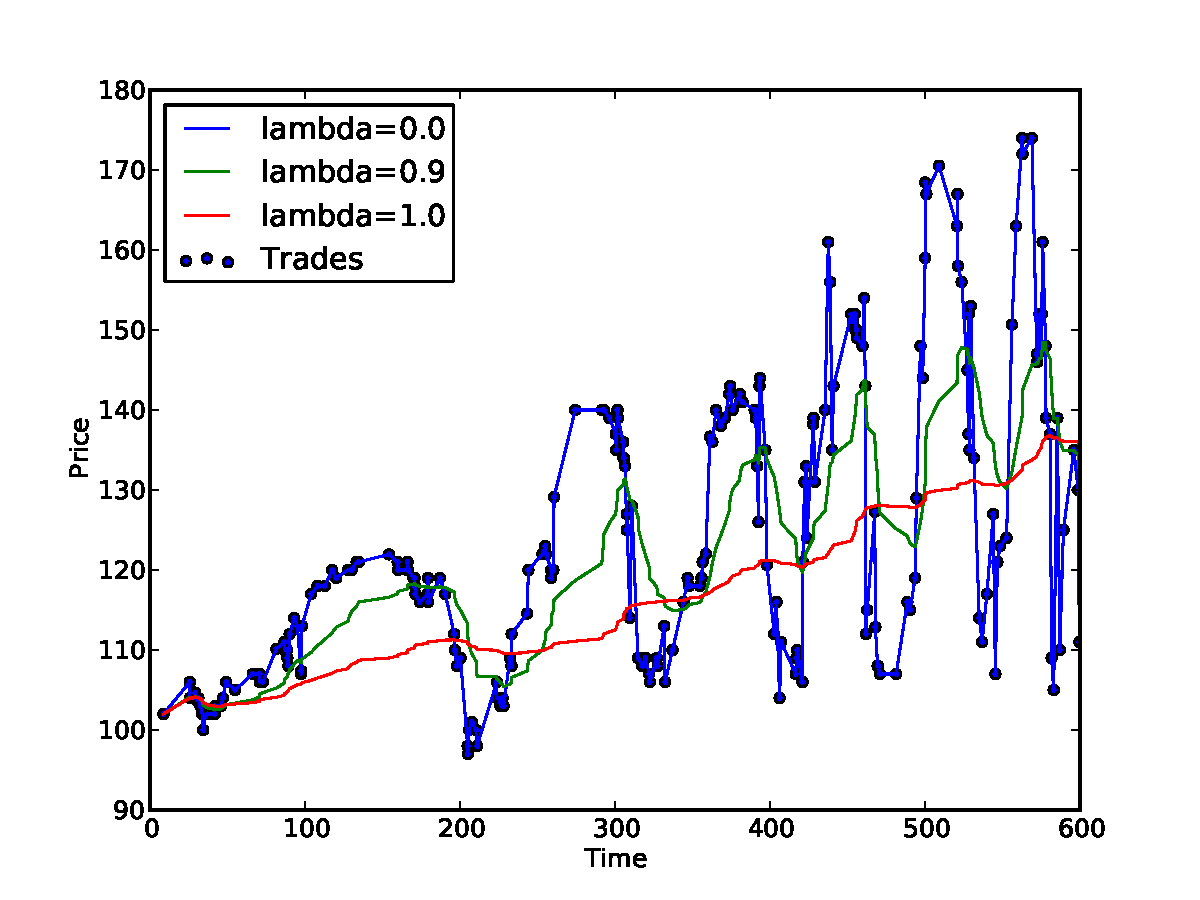
\includegraphics[width=\columnwidth]{graphs_and_stats/graph_equilibriums.pdf}
  \caption{The affect of the weighting value on the price equilibrium
  \label{fig:equilibrium}
  estimate.}
\end{figure}

The Adaptive Aggressive algorithm calculates the price of its shout by
computing a target price ($\tau$) which is dependent upon
the state of the market. However, before we can go into detail, we must define
two concepts: an intra-marginal trader is a trader that bids above the
equilibrium if they are a buyer (or asks below the equilibrium if they are a
seller) whereas an extra-marginal trader will never trade above the
equilibrium if they are a buyer (or below the equilibrium if they are a
seller).

Whether our trader is acting in an intra-marginal or extra-marginal capacity
will depend upon the limit price for our order. If we have a limit price above
the equilibrium (below the equilibrium for a seller) then we act as an
intra-marginal trader otherwise we act as an extra-marginal trader. The
difference is illustrated in Figure \ref{fig:r_price}

\begin{figure}[H]
\centering
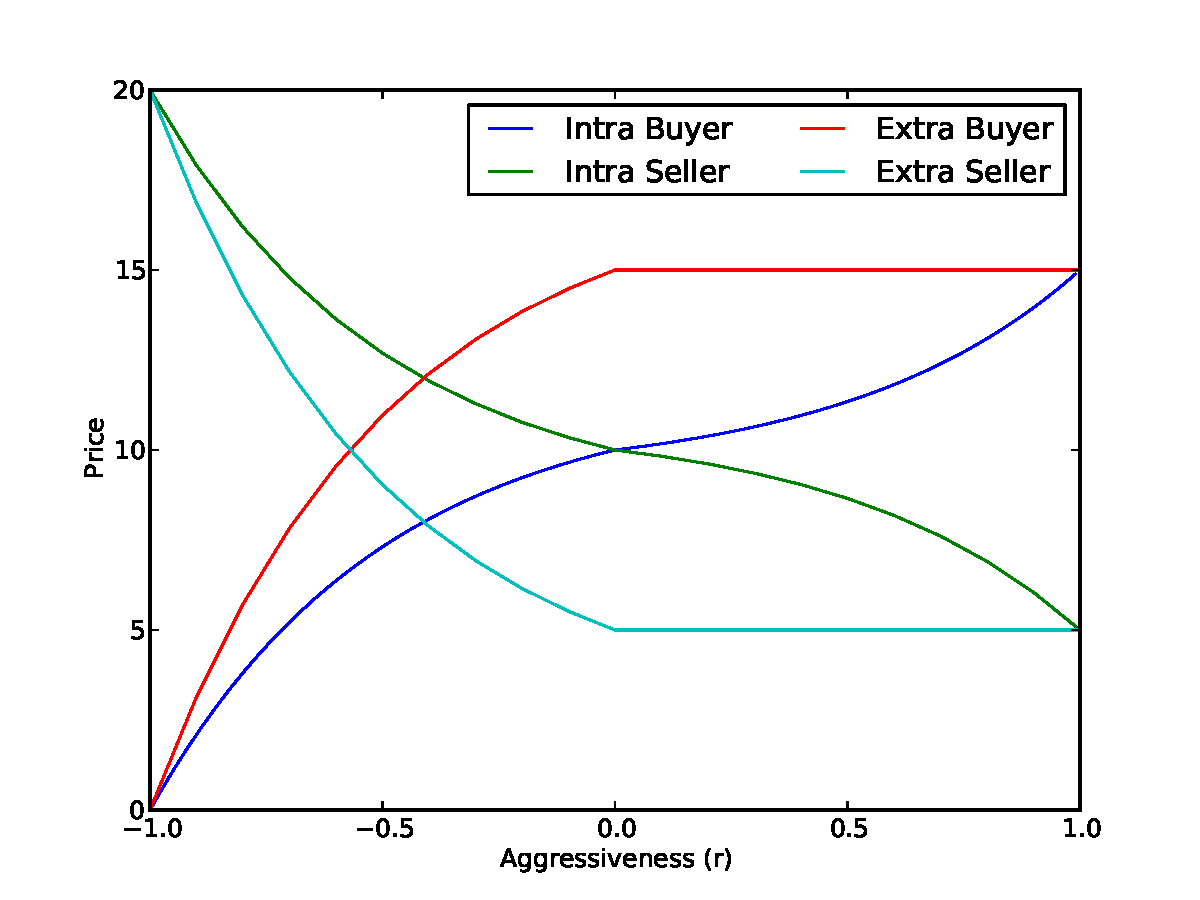
\includegraphics[width=\columnwidth]{graphs_and_stats/graph_r.pdf}
\caption{Aggressiveness price relationship}
\label{fig:r_price}
\end{figure}

The price that we then submit will depend upon which capacity we are acting
under, based on the follow equations.

\textbf{Intra-marginal buyer}
\begin{equation}
    \tau =
    \begin{cases}
        \hat{p}^*(1- \frac{e^{-r\theta}-1}{e^{\theta}-1}) &  \text{if r } \in (-1,0)  \\
        \hat{p}^* + (l_i-\hat{p}^*)(\frac{e^{r\theta}-1}{e^\theta-1}) & \text{if r} \in (0,1)
    \end{cases}
    \label{eqn:intrabuyer}
\end{equation}
where $\theta$ (Section \ref{sec:AA_long_term_learning}) measures the volatility of the
market, $l_i$ is the limit price for the buyer, and $\hat{p}^*$ is the estimator of the
equilibrium price.

\textbf{Extra-marginal buyer}
\begin{equation}
    \tau =
    \begin{cases}
        l_i(1-\frac{e^{-r\theta}-1}{e^\theta-1}) &  \text{if r } \in (-1,0)  \\
        l_i & \text{if r } \in (0,1)
    \end{cases}
    \label{eqn:extrabuyer}
\end{equation}

\textbf{Intra-marginal seller}
\begin{equation}
    \tau =
    \begin{cases}
        \hat{p}^* + (\text{MAX}-\hat{p}^*)( \frac{e^{-r\theta}-1}{e^{\theta}-1}) &  \text{if r } \in (-1,0)  \\
        c_j + (\hat{p}^*-c_j)(1-\frac{e^{r\theta}-1}{e^\theta-1}) & \text{if r } \in (0,1)
    \end{cases}
    \label{eqn:intraseller}
\end{equation}
where MAX is the maximum value that can be submitted to the market and $c_j$ is
the limit price for the seller.

\textbf{Extra-marginal seller}
\begin{equation}
    \tau =
    \begin{cases}
        c_j + (\text{MAX}-c_j)(1-\frac{e^{-r\theta}-1}{e^\theta-1}) &  \text{if r } \in (-1,0)  \\
        c_j & \text{if r } \in (0,1)
    \end{cases}
    \label{eqn:extraseller}
\end{equation}

In the paper\cite{AA_thesis}, there was a different value used instead of $\theta$, designed to
ensure that the curve produced by the equations was continuous. However, we
found that just using $\theta$ was still sufficiently accurate and greatly
simplified the above equations.

% TODO Jonny and Rupe proof read

One of the equations is then used to determine the ideal price that we want to
be trading at. We then use the following rules to determine the actual shout
that we will make when asked to submit a new order. The $o_{bid}$ and $o_{ask}$
represent the best (highest) bid and best (lowest) ask on the market that have
not yet been accepted. The value of $\eta$ is set as a parameter and reflects
how quickly we converge on our estimated price (higher $\eta$ converge slower).

%\textbf{Bidding rules for buyer:}
\begin{algorithm}[H]
    \caption{Bidding rules for buyer}
    \begin{algorithmic}
        \IF{$l_i \leq o_{bid}$}
            \STATE submit no bid (market transacting above our limit).
        \ELSE
            \STATE submit bid given by $bid_i = \textstyle o_{bid} + \frac{\textstyle \tau - o_{bid}}{\textstyle \eta}$.
        \ENDIF
    \end{algorithmic}
    \label{alg:bidding_rules_buyer}
\end{algorithm}

%\textbf{Bidding rules for seller:}
\begin{algorithm}[H]
    \caption{Bidding rules for seller}
    \begin{algorithmic}
        \IF{$c_j \geq o_{ask}$}
            \STATE submit no ask (market transacting below our limit).
        \ELSE
            \STATE submit ask given by $ask_i = \textstyle o_{ask} - \frac{\textstyle o_{ask}-\tau}{\textstyle \eta}$.
        \ENDIF
    \end{algorithmic}
    \label{alg:bidding_rules_seller}
\end{algorithm}

Since these all require an existing bid on the market, there were different
rules that were used to determine what shout to make if we were the first
trader selected to make a bid. These can be found in the Adaptive Aggressive
paper \cite[p.~32]{AA_paper} but are not defined here.

Initially when we ran our algorithm we found that it was occasionally making a
loss upon receiving a new order from the scheduler containing a different limit
price. This was because our previous bids had been submitted using
the limit price from the previous order (which may be outside the range
we are now allowed to trade within). Since on the Bristol Stock Exchange it
is not possible to remove a bid, we added additional logic to notify us of the
new order. If it was found that the new order contained a limit that was
outside of our trading range, we cleared our previous bid using a stub.


\subsubsection{Short term learning} \label{sec:AA_short_term_learning}
% OWNER: Max
% - Graphs - r vs price equilibrium.
The aggressiveness of the Adaptive Aggressive algorithm is updated at every
time step using Equation \ref{eqn:update_aggressive} based on the following rules.

%\textbf{Learning rules for buyer:}
\begin{algorithm}[H]
  \caption{Learning rules for buyer}
  \begin{algorithmic}
    \IF{trade occurs at price $q$}
        \IF{$\tau \geq q$}
            \STATE be less aggressive (our price too high).
        \ELSE
            \STATE be more aggressive (our price too low).
        \ENDIF
    \ELSIF{ $\tau \leq o_{bid}$ }
        \STATE be more aggressive (our price too low).
    \ENDIF
  \end{algorithmic}
  \label{alg:learning_rules_buyer}
\end{algorithm}

%\textbf{Learning rules for seller:}
\begin{algorithm}[H]
  \caption{Learning rules for seller}
  \begin{algorithmic}
    \IF{trade occurs at price $q$}
        \IF{$\tau \leq q$}
            \STATE be less aggressive (our price too low).
        \ELSE
            \STATE be more aggressive (our price too high).
        \ENDIF
    \ELSIF{ $\tau \geq o_{bid}$ }
        \STATE be more aggressive (our price too high).
    \ENDIF
  \end{algorithmic}
  \label{alg:learning_rules_seller}
\end{algorithm}

\begin{equation}
  \begin{aligned}
    r(t+1) &= r(t) + \beta_1(\delta(t) - r(t))\\
    \delta(t) &= (1 \pm \lambda_r)r_{shout} \pm \lambda_a
  \end{aligned}
  \label{eqn:update_aggressive}
\end{equation}

$\delta(r)$ is our target aggressiveness which is slightly above or below
(depending on the situation) $r_{shout}$, the value of
aggressiveness that would give us the current best outstanding shout. The value
of $r_{shout}$ was computed by reversing the equations found in
\ref{sec:AA_price_estimation} (an example can be seen in Equation
\ref{eqn:reverse_intra_buyer} for calculating the reverse of the intra-marginal
buyer). The rate at which we converged on the desired aggressiveness is
determined by $\beta_1$. The affect different $\beta_1$ values have on
performance is explored in Section \ref{sec:calibration_beta}.

$\lambda_r$ and $\lambda_a$ represent the relative and absolute change in
$r$ respectively. The absolute change exists to prevent $r$ from never being able
to update from a value of 0. Depending on the rules above, we either set the
two values to positive to become more aggressive or negative to become less
aggressive.


\begin{equation}
r_{shout}=
\begin{cases}
 -ln\left(\frac{ (1-\frac{\tau}{\hat p^*}) (e^\theta-1) + 1}{\theta}\right) & \tau
< \hat p^*\\
ln\left( \frac{(e^\theta -1) (\frac{\tau - \hat p^*}{l_i - \hat p^*} + 1)
}{\theta} \right)&
\textstyle{otherwise}
\end{cases}
\label{eqn:reverse_intra_buyer}
\end{equation}

The aggressiveness is dependent on our limit price and the current market state as
is illustrated in Figure \ref{fig:avtime}. In order to collect more data, we
increased the scheduler to distribute orders every five timesteps instead of
every thirty. This increases the number of trades in the market which in turn
provides us with a far more accurate estimate of the price equilibrium and more
trading data to work with.

One of the first conclusions we can draw from the graph is that our trader is
always playing an active role in the market, that is they are trading above the
market equilibrium. The reason for this is that the scheduler was set to
periodic meaning that the limit prices were provided in order to create the
sine wave visible in Figure \ref{fig:avtime}. Therefore, everyone receives limit
prices close to each other meaning that we have a competitive market which
means we have to trade close to our limit price. This is further reinforced by
the short order duration making it difficult to wait for a trade.

Initially our trader has a lower aggressiveness value (close to zero), this is
because the trader lacks information about the market and therefore adopts a
more passive role to prevent selling far above the equilibrium

The dips in the aggressiveness correspond to the falling equilibrium price
where we can afford to trade further below our limit because the gap between
our limit price and the market equilibrium is increasing.


\begin{figure}[H] 
\centering
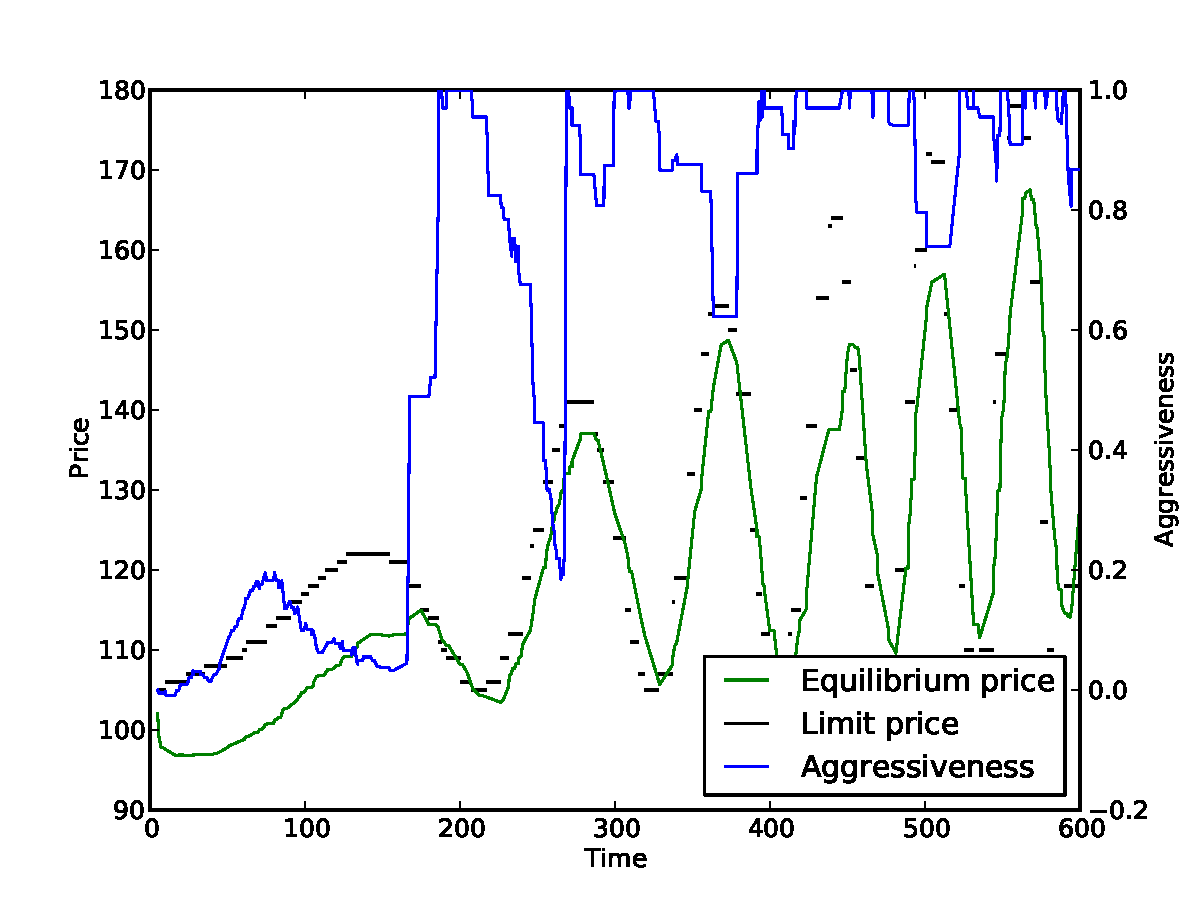
\includegraphics[width=\columnwidth]{graphs_and_stats/graph_aggressiveness_vs_price.pdf}
\caption{Aggressive and Price equilibrium throughout a trading day for an AA
buyer}
\label{fig:avtime}
\end{figure}

\subsubsection{Long term learning} \label{sec:AA_long_term_learning}
% OWNER: Max
% - theta
The Adaptive Aggressive algorithm incorporates a long term learning component
that is affected by the volatility of the market. In order to do this we create
a measure of the market volatility, $\theta$, which is then updated every
timestep using Equation \ref{eqn:update_theta}. The value of $\theta^*(\alpha)$
represents the value of $\theta$ that will allow us to act optimally in a
market with a volatility of $\alpha$. This value of $\theta^*$ is scaled with
respect to a minimum and maximum theta, constants that are hard coded into the
function (we used -8 and 2 respectively), to keep it within a certain range.
We then moved towards this desired value of $\theta^*$ at a rate that is
determined by $\beta_2$. The larger value of $\beta_2$ the faster we converged
towards $\theta^*$. We initially set the learning rate at 0.5, however the 

The $\alpha$ (see Equation
\ref{eqn:alpha}) is measure of the volatility of the market which is calculated
by looking at the variance of the last N trades around the market equilibrium.
So if the majority of trades are close to the equilibrium price then we are in
a stable market and vice versa.. The $\alpha_{max}$ and $\alpha_{min}$
represent the a largest and smallest market volatility to date (these are
initialised to 0.02 and 0.15 respectively).

\begin{figure}
  \centering
  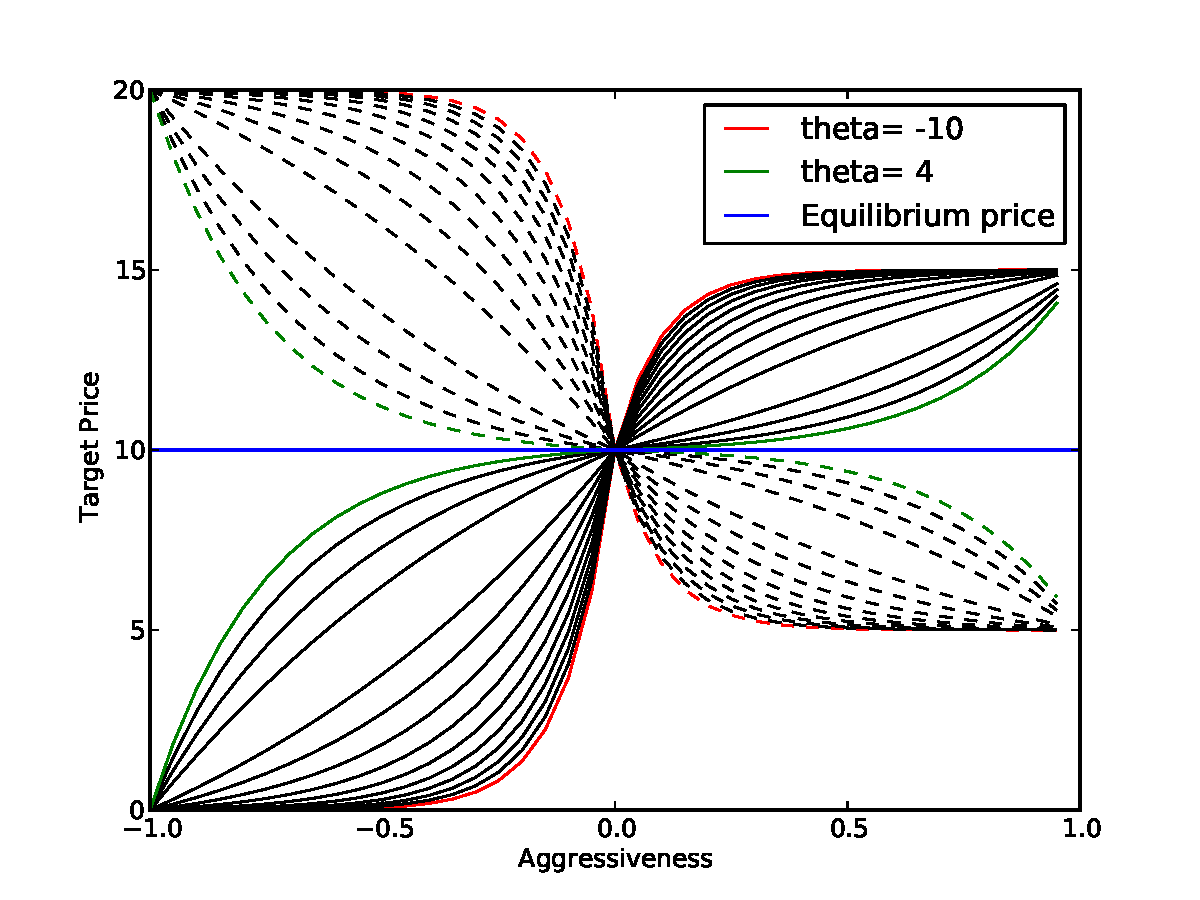
\includegraphics[width=\columnwidth]{graphs_and_stats/graph_thetas.pdf}
  \caption{How different thetas affect the target price calculations}
  \label{fig:theta}
\end{figure}

The $\theta$ affects the degree to which changing the aggressiveness moves the
target price  away from the equilibrium. So a high value of $\theta$ means that a
relatively small change in aggressiveness will result in a large move away from
the equilibrium price. This is illustrated in Fig. \ref{fig:theta}, when
$\theta=4$, between aggressiveness of -0.5 and 0.5, the price stays very close
to the equilibrium.

The graph in Fig \ref{fig:theta_v_time} represents our value of theta
throughout the trading day. It peaks at the beginning of the market session
when the market is most stable then decreases as the market begins to
oscillate.

\begin{figure}
  \centering
  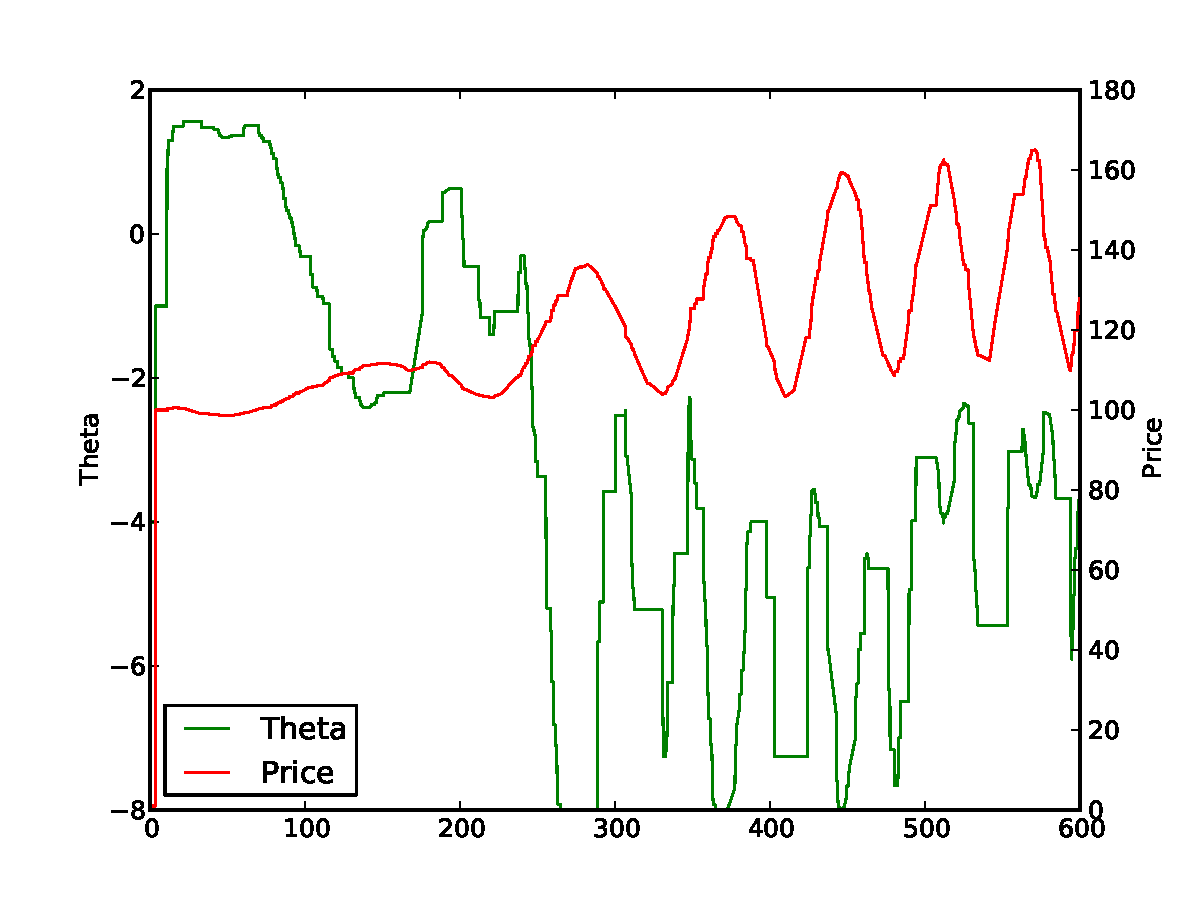
\includegraphics[width=\columnwidth]{graphs_and_stats/graph_theta_vs_time.pdf}
  \caption{How theta varies across a market day}
  \label{fig:theta_v_time}
\end{figure}

%\begin{figure} 
%\centering
%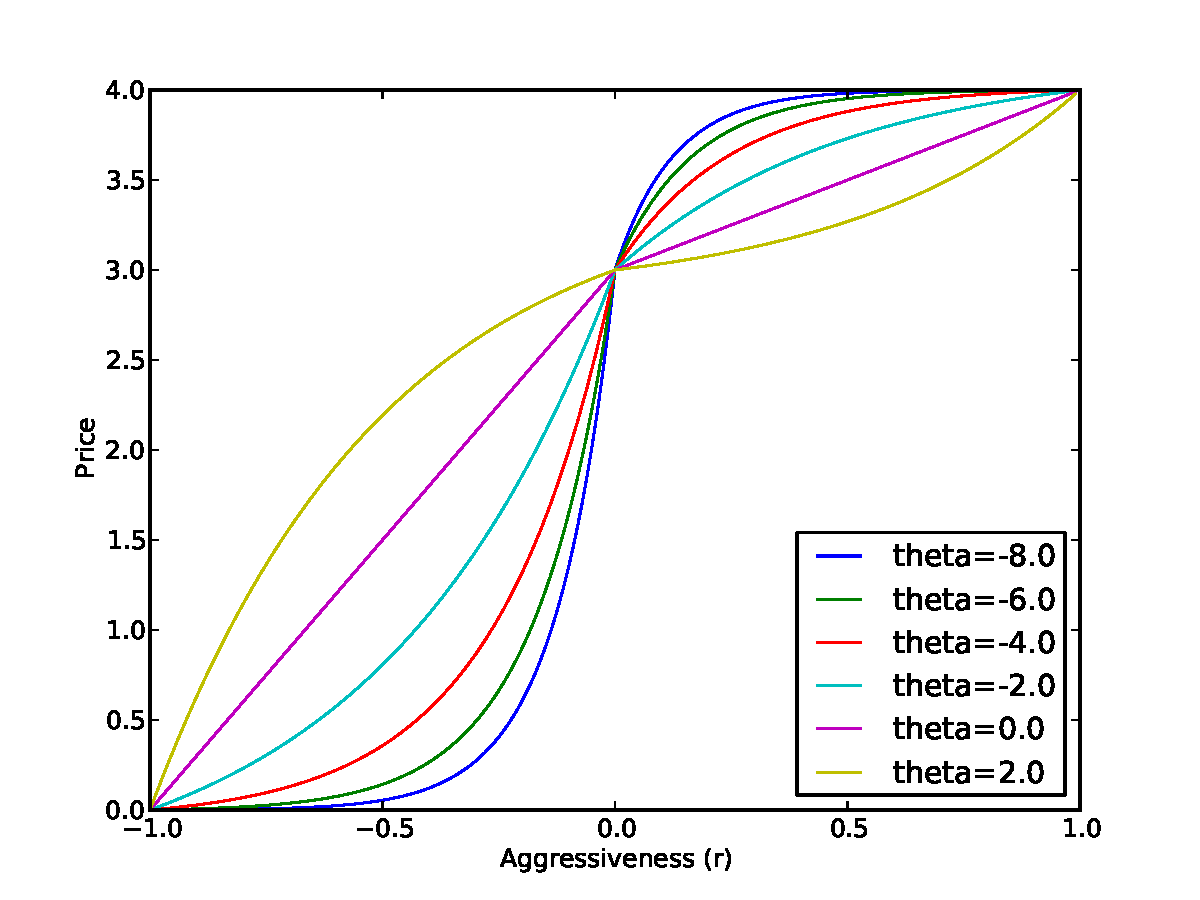
\includegraphics[width=\columnwidth]{graphs_and_stats/graph_intra_buyer_thetas.pdf}
%\caption{Intra buyer thetas}
%\end{figure}

\begin{equation}
  \theta(t+1)=\theta(t)+\beta_2(\theta^*(\alpha)-\theta_t)\\\\
  \label{eqn:update_theta}
\end{equation}

\begin{equation}
  \alpha = \frac{\sqrt{\frac 1 N \sum^T_{i=T-N+1}(p_i-\hat p^*)^2}}{\hat p^*}
  \label{eqn:alpha}
\end{equation}

\begin{equation}
  \theta^*(\alpha) = (\theta_{max}-\theta_{min})
  \left(\frac{1-e^{\gamma\left(\frac{(\alpha-\alpha_{min})}{(\alpha_{max}
  -\alpha_{min})}-1\right)}}{1-e^{-\gamma}}\right)
  \label{thetastar}
\end{equation}


\section{Calibration} \label{sec:calibration}
% OWNER: Group
% - $\beta_1$, $\beta_2$, $\gamma$, $\eta$
% - potential to compare statistically?
\subsection{$\eta$ parameter} \label{sec:calibration_eta}
The $\eta$ value in the AA bidding function determines how quickly the shout
price moves towards from the best shout to the calculated target price. A
higher value of $\eta$ will reduce the rate of change making the trader slower
to react to market events. This is confirmed by our tests. A trader with $\eta
= 1000$ makes an average profit of 94.507 over 100 trades. Another trader with
a lower $\eta = 100$ makes a higher average profit of 116.553. Using $\eta = 3$
from the AA thesis \cite{AA_thesis} gives a profit of 136.555. So clearly it is important for the
shout price to respond to quickly up the changing market. Setting $\eta$ too
low would cause outlier trades to have a significant impact which would reduce
the margins.


\subsection{$\beta_1$ and $\beta_2$ parameters} \label{sec:calibration_beta}

We update our aggressiveness and theta values more often than in the original
Adaptive Aggressiveness paper \cite{AA_thesis}. This is advantageous since it
allows us to update to rapidly changing market conditions. Since we update
these values more often the learning rates have to be comparatively lower
otherwise the algorithm will effectively learn immediately. We ran tests over
four thousand market sessions with various different values of $\beta_1$ (which
controls the rate of change of aggressiveness) and $\beta_2$ which controls the
rate of change of theta, the results are shown in Table \ref{tbl:beta_results}.
The average profit made by the Adaptive Aggressive algorithm did not appear to
be heavily affected by the variation in either of the two $\beta$ values.
However, if we set the value of $\beta_1$ to zero then we have a marked drop in
performance, this is because the aggressiveness will not change and our
algorithm will not be able to adapt to changing market conditions. Although a
value of zero for $\beta_2$ does not appear to have a significant effect. This
is because we initalise $\theta$ to -4 which is a fairly accurate model of our
environment. \textbf{RUPERT PUT THE THETA=2 RESULTS HERE}
%TODO
\begin{table}[H]
  \centering
  \begin{tabular}{ | c | C{2.7cm} | C{2.7cm} | }
    \hline
    \multirow{2}{*}{\textbf{Value ($v$)}} & \multicolumn{2}{ c | }{\textbf{Average finishing balance (3 dp.)}} \\
    & $\beta_1 = v, ~ \beta_2 = 0.5$ & $\beta_1 = 0.5, ~ \beta_2 = v$ \\
    \hline
        0.00 & 109.388 & 128.071 \\
        0.01 & 127.431 & 128.212 \\
        0.02 & 128.318 & 128.157 \\
        0.03 & 128.971 & 128.366 \\
        0.04 & 129.551 & 128.177 \\
        0.05 & 129.666 & 128.088 \\
        0.06 & 129.864 & 128.308 \\
        0.07 & 129.797 & 128.000 \\
        0.08 & 129.698 & 128.100 \\
        0.09 & 130.170 & 128.173 \\
        0.10 & 129.138 & 128.903 \\
        0.20 & 129.038 & 129.287 \\
        0.30 & 129.312 & 129.376 \\
        0.40 & 129.230 & 129.344 \\
        0.50 & 129.467 & 129.081 \\
        0.60 & 129.062 & 129.187 \\
        0.70 & 129.164 & 128.947 \\
        0.80 & 129.137 & 129.144 \\
        0.90 & 129.271 & 129.405 \\
        1.00 & 129.286 & 129.368 \\
    \hline \hline
    ZIC & \multicolumn{2}{ c | }{ 89.030} \\
    ZIP & \multicolumn{2}{ c | }{117.461} \\
    \hline
  \end{tabular}
  \caption{Difference in finishing balance with respect to change in $\beta_1$ and $\beta_2$ values.}
  \label{tbl:beta_results}
\end{table}

\subsection{$\lambda$ parameter} \label{sec:calibration_lambda}
We tested $\lambda$ values from $0$ to $1$ in $0.1$ increments over 8000
market sessions (of 600 timesteps each) to find their effect on AA's
performance. We didn't find any statistically significant difference between
the different values. 

\begin{table}[H]
  \centering
  \begin{tabular}{ | c | c | }
    \hline
    \textbf{$\lambda$ value} & \textbf{Average finishing balance (3 dp.)} \\
    \hline
        0.0 & 128.048 \\
        0.1 & 128.040 \\
        0.2 & 128.041 \\
        0.3 & 128.314 \\
        0.4 & 128.268 \\
        0.5 & 128.278 \\
        0.6 & 128.224 \\
        0.7 & 128.380 \\
        0.8 & 128.172 \\
        0.9 & 128.365 \\
        1.0 & 128.462 \\
    \hline \hline
        ZIC &  89.521 \\
        ZIP & 116.719 \\
    \hline
  \end{tabular}
  \caption{Difference in finishing balance with respect to change in $\lambda$.}
  \label{tbl:lambda_results}
\end{table}


\section{Results} \label{sec:results}
% OWNER: Group
% - Graph: Average balance over time
% - Statistical analysis - why you used a certain test
%   Ed's report: ``According to the conducted Wilcoxon-Mann-Whitney two-tailed rank-sum tests, the difference in the observed efficiencies is significant ($U = 2, N_1 = N_2 = 10, p < 0.0003$)."
% - Experiment with changing scheduler
% - Other graphs

\begin{table}[H]
  \centering
  \begin{tabular}{ | c | C{2.5cm} | C{2.5cm} | }
    \hline
    \multirow{2}{*}{\textbf{Strategy}} & \multicolumn{2}{c|}{\textbf{Average
    finishing balance (3 dp.)}} \\
%    \cline{2-3}
%    & \vspace{0.05cm} Fixed & \vspace{0.05cm} Jittered \\
    & Fixed & Jittered \\
    \hline
    ZIC & 93.863 & 93.713 \\
    SHVR & 106.139 & 106.270  \\
    ZIP & 120.434 & 120.543 \\
    AA & 136.555 & 136.428 \\
    \hline
  \end{tabular}
  \caption{Average balances for different trading strategies.}
  \label{tbl:results}
\end{table}

We ran 22750 market sessions with AA, SHVR, ZIC and ZIP traders (half
buyers, half sellers). For each ratio 50 market sessions were run. The Wilcoxon
signed-rank test was used to evaluate the significance of the results. The null
hypothesis is that the difference between the pairs of traders is zero. For
each trader paired with AA we can reject the null hypothesis ($p < 2.2 \cdot
10^{-308}$). The results using fixed and jittered price generation were
virtually identical.

\begin{figure}[H]
  \centering
  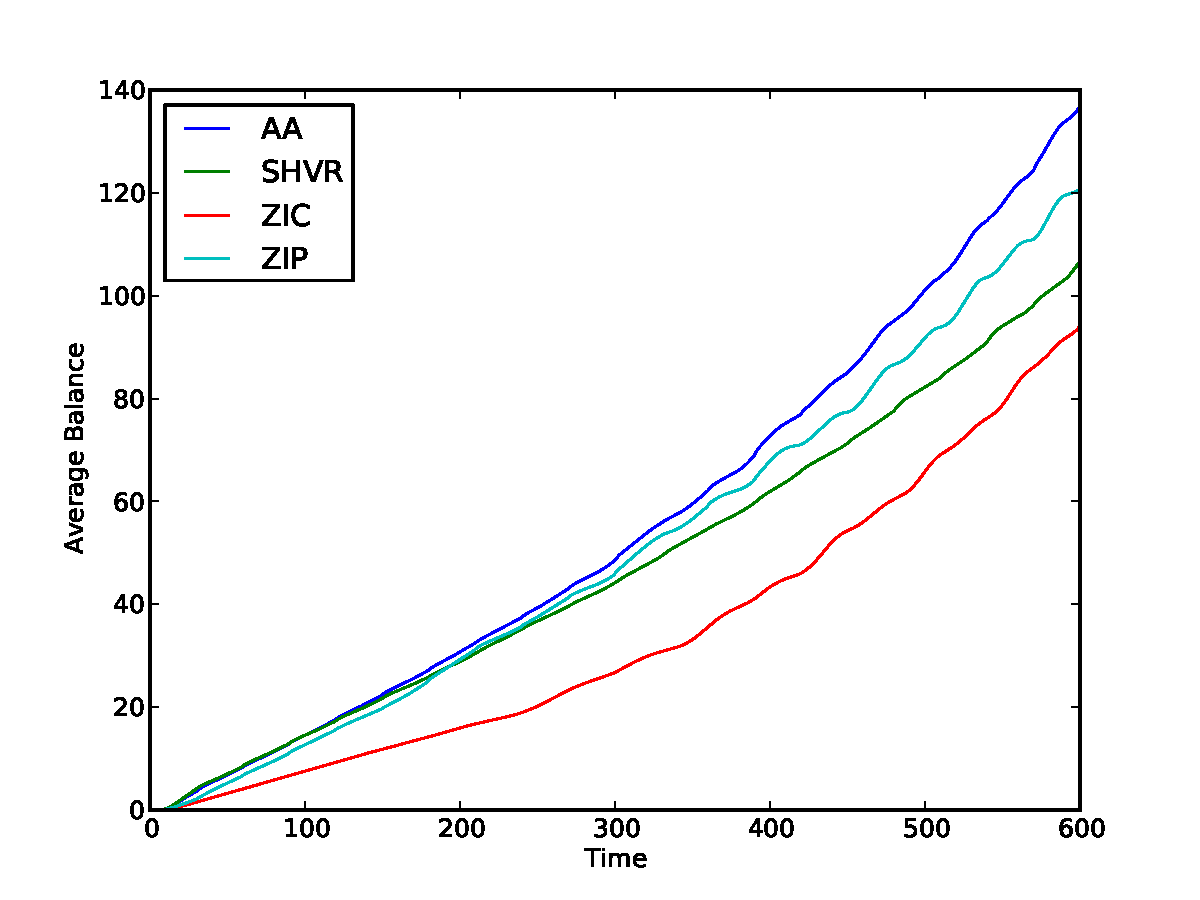
\includegraphics[width=\columnwidth]{graphs_and_stats/graph_average_balance_vs_time.pdf}
  \caption{Average balance over 22750 trials.}
  \label{fig:average_balance_vs_time}
\end{figure}

Figure \ref{fig:average_balance_vs_time} shows that AA consistently makes more profit.

\begin{table}[H]
  \centering
  \begin{tabular}{ | c | c | }
    \hline
    Strategy & Average finishing balance (3 dp.) \\
    \hline
    ZIP & 110.006 \\
    AA & 136.378 \\
    \hline
  \end{tabular}
  \caption{Market session with just AA and ZIP traders.}
  \label{tbl:two_traders}
\end{table}

We ran the Wilcoxon signed-rank test on the values in Table
\ref{tbl:two_traders} which resulted in $p < 2.2 \cdot 10^{-308}$. The AA
traders outperformed the ZIP traders 99.66\% of the time. ZIP performs worse in
a market with just AA traders which suggests ZIP was reliant on trades with the
ZIC and SHVR traders.

% TODO: Big graph of time and price

\section{Conclusion} \label{sec:conclusion}
% OWNER: Group
% - Thank you and good night
% - Hold for applause
Text.\\

\bibliographystyle{unsrt}
\bibliography{algo_report}
\end{document}
